\chapter{Atacuri Spectre}

\emph{Spectre} \cite{spectre2019} este o clasă de atacuri asemănătoare cu
\emph{Meltdown}, care exploatează efectele secundare ale execuției speculative
pentru a extrage informații în mod malițios din spațiul de memorie al unei
victime. La nivel înalt, se bazează pe găsirea sau introducerea unei secvențe
de instrucțiuni în spațiul de adrese al procesului victimă. Mai apoi, execuția
acestei secvențe va crea un canal de comunicare ascuns prin care sunt transmise
date din spațiul de memorie al victimei către atacator. Similar cu
\emph{Meltdown} \cite{meltdown2018}, atacul nu se bazează pe niciun fel de
vulnerabilitate software, ci abuzează vulnerabilități microarhitecturale la
nivel hardware. Chiar dacă în urma executării speculative a unei secvențe de
instrucțiuni, se revine la o stare anterioară, schimbările apărute pe parcus la
nivel de cache pot persista, aceasta fiind vulnerabilitatea principală.

În acest capitol se vor prezenta cele două variante principale din clasa de
atacuri Spectre. În ultimul capitol va fi descrisă o implementare demonstrativă
a variantei 1, care exploatează o zona de memorie partajată cu procesul
victimă.

\section{Diferențe față de Meltdown}

Prima diferență față de \emph{Meltdown} este că variantele \emph{Spectre} evită
provocarea unei excepții prin accesul ilegal al unei zone de memorie. În
schimb, se bazează ori pe antrenarea \emph{branch-predictor-ului} ori pe
injectarea unor adrese alese special în \emph{branch-target-buffer} cu scopul
de a accesa zona de memorie de interes, doar în mod speculativ. Astfel, nu este
necesară gestionarea excepțiilor, atacul interferând minimal, chiar insesizabil,
cu executarea normală a programului.

A doua diferență constă în faptul că \emph{Meltdown} exploatează o
vulnerabilitate specifică procesoarelor \emph{Intel} și câtorva procesoare
\emph{ARM} prin intermediul cărora instrucțiuni executate speculativ pot ignora
restricțiile impuse de bitul \emph{user/supervisor} prezent în intrările din
tabelele de traducere ale adreselor virtuale. Astfel, \emph{Meltdown} poate
accesa memoria Kernel și implicit poate citi toată memoria fizică a sistemului
prin intermediul unui canal ascuns. \emph{Spectre}, în schimb extrage prin
intermediul unei zone de memorie partajată și a unui canal ascuns implementat
în zona respectivă de memorie, doar informații la care victima țintă are acces.
Se încalcă astfel izolarea inter-proces, dar nu se poate accesa direct zona de
Kernel.

Spre deosebire de \emph{Meltdown}, atacurile \emph{Spectre} afectează o plajă
mult mai largă de arhitecturi și s-au dovedit a fi mai dificile de mitigat. Mai
mult, mecanismul care stă la baza mitigarii \emph{Meltdown} (KAISER
\cite{gruss2017kaslr}) nu protejează în niciun fel împotrivă variantelor
\emph{Spectre}.

\section{Spectre V1}
\label{sec:spectrev1}

Varianta întâi de \emph{Spectre} presupune manipularea
\emph{branch-predictor-ului} \ref{sec:branch_prediction} în prezicerea eronată
a ramurii de execuție în cadrul unei structuri decizionale. Astfel, prin
intermediul execuției speculative un atacator poate citi zone arbitrare de
memorie din afara contextului său de execuție, ceea ce încalcă principiile de
izolare impuse de memoria virtuală și sistemul de operare. 

\subsection{Descrierea Atacului}

O secvență de cod precum \ref{code:conditional} se poate regăsi în cadrul unui
apel de funcție (e.g. funcție de sistem sau parte dintr-o bibliotecă), care
primește ca argument o variabilă dintr-o sursă oarecare, neverificată (e.g. în
urma unui apel către un API). Să considerăm situația în care procesul care
rulează codul respectiv (i.e. victima) are acces la un tablou cu elemente de
tip byte \texttt{array} de dimensiune \texttt{array\_size} și la tabloul cu
același tip de elemente, \texttt{probe} de dimensiune $256 * 4096 = 1MB$.
Verificarea de la începutul secvenței de cod are rol în securizarea
programului. În eventualitatea rulării secvenței cu o valoare în \texttt{x} mai
mare sau egală cu \texttt{array\_size} să se evite declanșarea unei excepții
(e.g. \emph{Segmentation Fault}), sau a accesării unei alte zone de memorie din
cadrul de execuție a procesului victimă (e.g. dacă valoarea din x reprezintă
diferența dintre adresa de început a tabloului \texttt{array} și adresa de
început a unui alt tablou \texttt{secret}).

\begin{lstlisting}[language=c, label=code:conditional,
                    caption=Executarea speculativă în structura decizională]
  if (x < array_size) {
    /* prin executarea speculativa putem accesa date din afara
       tabloului array fara declansarea unei exceptii */
    data = probe[array[x] * 4096];
  }
\end{lstlisting}

Se consideră cazul în care \texttt{array\_size} nu este încărcat în cache.
Determinarea ramurii care va fi urmată de fluxul de execuție va fi semnificativ
întârziată din cauza cererii din \emph{DRAM} a valorii variabilei respective,
care precede evaluarea condiției logice. Pentru a nu stagna execuția și a ține
unități de lucru din \emph{CPU} inactive se realizează o presupunere informată ce
vizează ramura pe care urmează să continue execuția, prin intermediul \emph{BPU}
(vezi secțiunea \ref{sec:branch_prediction} și figura
\ref{fig:branch_prediction}). Urmând prezicerea se pot executa speculativ
instrucțiunile ce urmează.

\begin{figure}[ht]
	\centering
	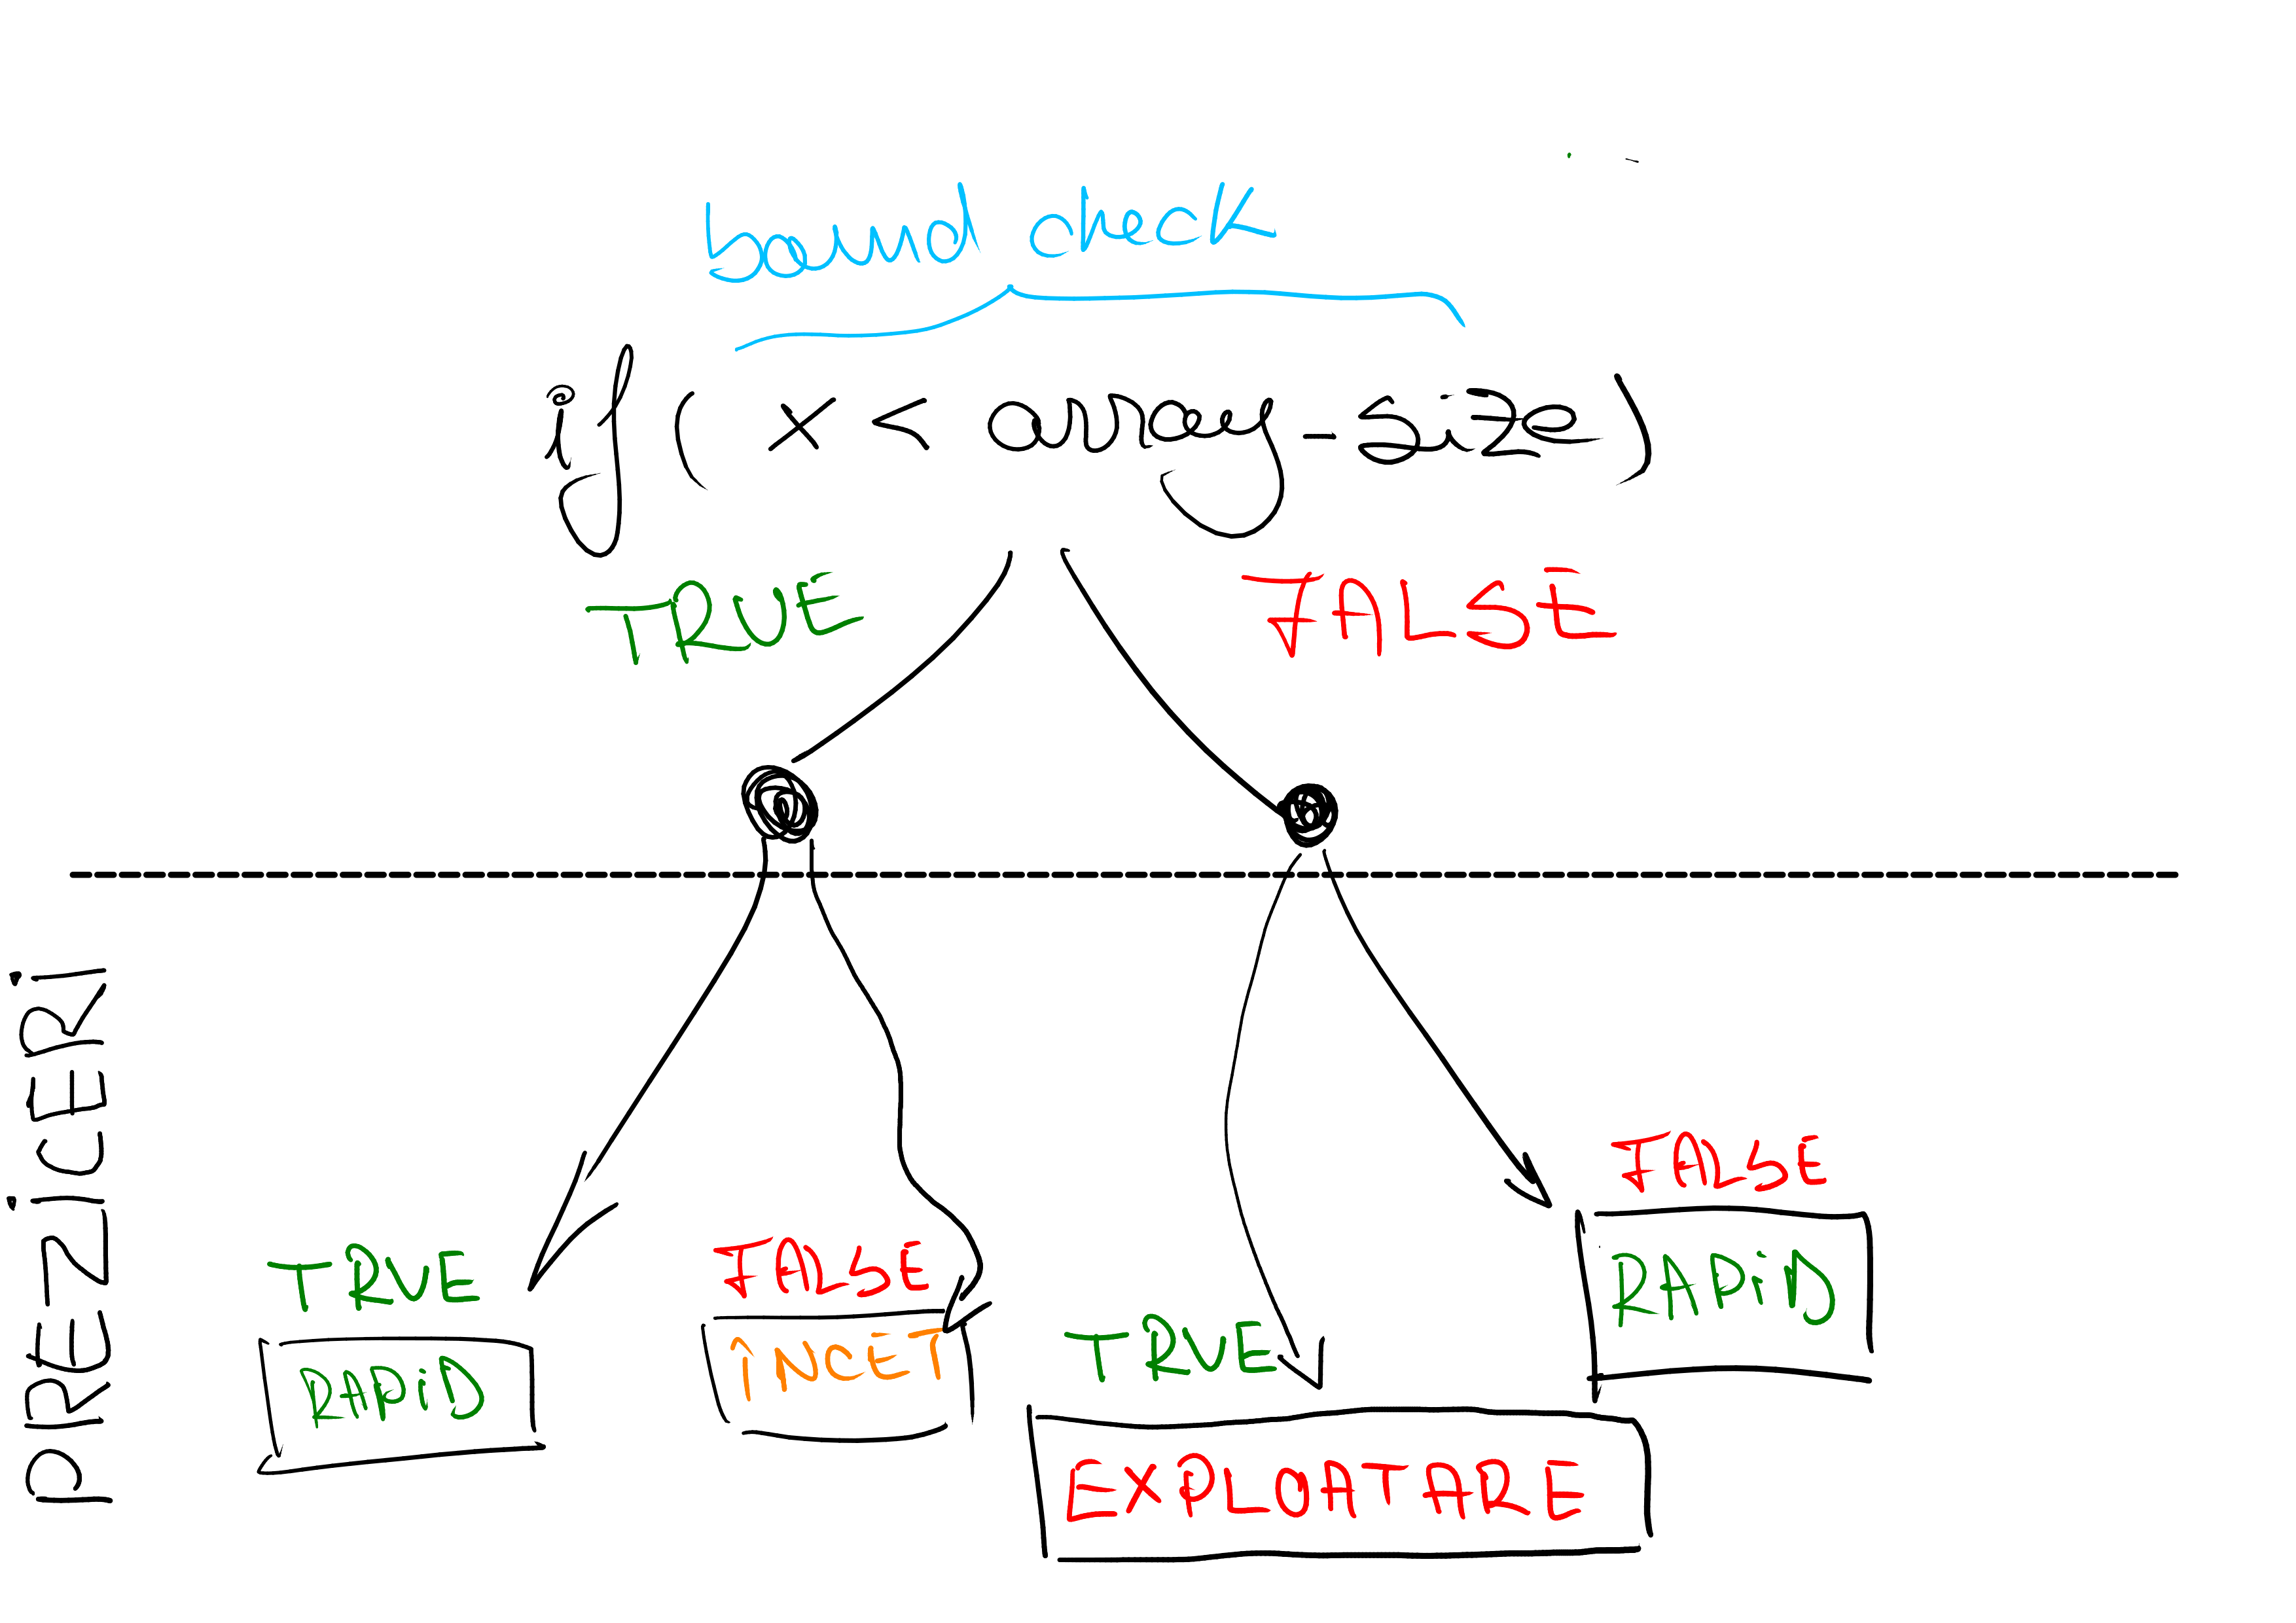
\includegraphics[width=0.9\textwidth]{images/branch_pred.png}
	\caption{Cele patru cazuri posibile în cadrul prezicerii unei ramuri.}
  \label{fig:branch_prediction}
\end{figure}

Acest tipar poate fi exploatat după cum urmează. Un atacator poate executa
intenționat în mod repetat zona respectivă de cod cu valori mai mici decât
\texttt{array\_size}. Astfel, la următoarea execuție a zonei respective,
\emph{BPU} va prezice că fluxul de execuție va urma prima ramură a structurii
decizionale (corespunzătoare evaluării condiției logice la \emph{True}). La
următoarea executarea a zonei respective atacatorul va transmite un \texttt{x}
cu o valoare malițioasă aleasă special în afara limitelor impuse de
\texttt{array\_size} ca în urma evaluării \texttt{array[x]} să întoarcă o
valoare \texttt{k} dintr-o alta zonă din spațiul de memorie al victimei.
Fereastra de timp poate fi suficient de mare ca \emph{linia 4} din
\ref{code:conditional} să fie executată speculativ. Astfel, va ajunge în cache
o linie din memorie corelată cu byte-ul \texttt{k} ce face parte din secretul
accesat speculativ. După ce valoarea din \texttt{array\_size} este primită din
\emph{DRAM}, iar condiția logică este evaluată la \emph{False}, starea CPU-ului
se întoarce la cea dinaintea executării speculative. \emph{Spectre},
exploatează faptul că în urma executării speculative eronate, la nivel
microarhitectural, starea cache-ului din \emph{CPU} nu este resetată.

Pentru finalizarea atacului și recuperarea datelor transmise pe canalul ascuns
se procedează ca în atacul \emph{Meltdown} (vezi \ref{sec:step_receive}). Se
utlizeaza tehnici precum \emph{FLUSH and RELOAD}, sau \emph{EVICT + TIME}
pentru a măsura timpul de acces în fiecare frame de $4KB$ din tabloul
\texttt{probe}. În cazul în care timpul de acces pentru variabila \texttt{k}
este seminificativ mai scăzut comparativ cu al celorlalte adrese, concluzionăm
că byte-ul de date tansmis corespunde cu valoarea \texttt{k} \cite{spectre2019}.

\subsection{Reproducerea atacului}

În practică, urmând strict detaliile descrise anterior, vom obține un nivel
scăzut de acuratețe. Deoarece comportamentul canalului de comunicare ascuns nu
este constant, ci fluctuează și executarea cu succes în mod speculativ a
instrucțiunilor dorite nu este garantată, este necesară repetarea pașilor de
multiple ori pentru fiecare byte, iar apoi determinarea statistică a valorii
celei mai probabile. 

S-a confirmat că această variantă a \emph{Spectre} afectează arhitecturile
\emph{Intel}, \emph{AMD Ryzen} cât și implementări \emph{ARM} care suportă
execuția speculativă. O variantă neoptimizată a atacului implementată în
limbajul \texttt{C} care este prezentată în lucrarea de cercetare
\cite{spectre2019} atinge viteze de $10$ KB/s pe un sistem cu un procesor
\emph{Intel\ i7-4650U}.

\subsubsection{Javascript}

Atacul s-a dovedit practic și în contextul browserelor web. S-a reușit
implementarea acestei variante a \emph{Spectre} în JavaScript și citirea unor
informații private în mod neprivilegiat din spațiul de memorie al procesului în
cadrul căruia rulează codul. Deoarece instrucțiunea \texttt{clflush} nu este
accesibilă prin intermediul limbajului acesta, se folosește o tehnică
alternativă precum \emph{EVICT and RELAOD}. De asemenea instrucțiunea
\texttt{rdtscp} nu este disponibilă, iar motorul din Chrome nu oferă un ceas de
mare precizie pentru a preveni \emph{timing attacks}. Pentru a depăși aceste
obstacole se poate construi un ceas cu precizie suficient de mare prin
incrementarea într-un thread separat a unei zone de memorie controlată de
atacator \cite{spectre2019}.

\subsubsection{Experimente personale}

Dezvoltând ideile anterioare am realizat o implementare personală care
ilustrează un scenariu mai realist în care atacatorul rulează un proces separat
de victimă și împarte cu aceasta doar o zonă de $1$MB de memorie partajată.
Implementarea cât și detaliile se găsesc în capitolul \ref{cap:poc}.

\section{Spectre V2}

Varianta a doua a clasei de atacuri \emph{Spectre} presupune otrăvirea
(\emph{poisoning}) salturilor indirecte (\emph{indirect branches}) (eg. o
instrucțiune de tip \texttt{jump} la o adresă reținută într-un registru). Un
atacator poate astfel determina execuția speculativă a unor instrucțiuni alese
special, prin tehnici care amintesc de ROP (\ref{sec:rop}), pentru accesarea și
apoi extragerea prin intermediul unui canal secret ale unor date accesibile
victimei.

\subsection{Descrierea atacului}

În momentul unui salt indirect, \emph{branch-predictor-ul} va încerca să
prezică adresa la care urmează să se continue execuția pentru a executa
speculativ în avans instrucțiunile ce urmează. În vasta majoritate a cazurilor
se obține o îmbunatățire a timpului de execuție a programului ca urmare a
acestei tehinici, deoarece timpul de recuperare a adresei de destinație poate
fi considerabil în cazul în care adresa de memorie nu este în cache-ul din
\emph{CPU}. Prezicerea se bazează pe istoricul adreselor accesate în trecut în
urma aceluiași salt indirect. Aceste date sunt reținute într-o structură numita
\emph{branch target buffer} și sunt codificate, în funcție de arhitectură, în
funcție de ultimii \texttt{k} biți ai adresei corespunzătoare.

\subsubsection{Antrenarea}

Atacul începe din contextul atacatorului. Acesta mimează salturile indirecte
executate în contextul victimei. Astfel se poate plasa un salt indirect în
contextul atacatorului la aceeași adresă virtuala la care se regăsește saltul
în contextul victimei, sau la o adresă care are în comun ultimii \texttt{k}
biți cu adresa corespunzătoare a victimei. Prin repetarea saltului la o adresă
aleasă de atacator aceasta va ajunge în \emph{branch target buffer}, iar
\emph{branch-predictor-ul} va fi antrenat să prezică că fluxul de execuție va
continua la adresa respectivă. Acest comportament depinde doar de adresa
virtuală și nu ia în considerarea \emph{PID-ul}, adresa fizică, etc. Astfel,
după antrenare, dacă în contextul victimei se execută saltul aferent, se vor
executa speculativ instrucțiuni începând cu adresa injectată de atacator.

S-a observat că atacatorul poate injecta chiar și adrese de memorie la care nu
are acces. Astfel, în contextul său pentru antrenare poate accesa direct adrese
ilegale, iar apoi să gestioneze eventualele excepții declanșate. În acest fel,
atacatorul poate alege orice adresă validă în contextul victimei, chiar dacă
nu are un corespondent valid în contextul său de execuție.

\begin{figure}[ht]
	\centering
	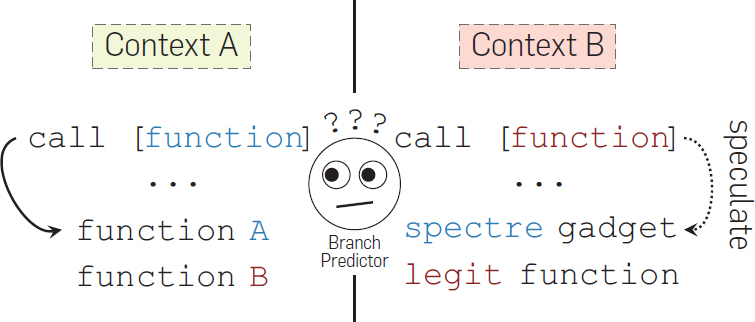
\includegraphics[width=0.9\textwidth]{images/branch_poisoning.jpg}
	\caption{Antrenarea branch-predictorului pentru a executa cod speculativ la 
           adrese alese special de către atacator \cite{spectre2019}.}
  \label{fig:branch_poisoning}
\end{figure}

\subsubsection{Alegerea adresei de destinație}

În urma saltului indirect victima va continua fluxul de execuție la adresa
injectată de atacator. Luând inspirație din atacurile de tip \emph{ROP}
(\ref{sec:rop}) putem alege o zonă de memorie în care începe un așa numit
\emph{Gadget Spectre}. Un \emph{Gadget Spectre} este o secvență de instrucțiuni
a cărei execuție va transmite informații private ale victimei, dorite de
atacator, printr-un canal secret.

Presupunând că victima are acces la doi registri \texttt{R1} și \texttt{R2}, un
gadget suficient ar trebuie să conțină două instrucțiuni după cum urmează.
Prima instrucțiune adună (scade, XOR-ează, înmulțește, etc.) adresa reținută în
registrul \texttt{R1} la registrul \texttt{R2}. A doua instrucțiune accesează
valoarea de la adresa registrului \texttt{R2}. Un atcator va deține în acest
scenariu controlul asupra adresei de memorie accesată (prin intermediul
\texttt{R1}) și asupra modului în care zona de memorie dorită este asociată
la o altă adresă citită prin intermediul \texttt{R2}.

Gadget-urile folosite trebuie să facă parte din zona executabilă din contextul
victimei pentru a garanta execuția speculativă a acestora în \emph{CPU}. 
Gadget-urile pot fi astfel alese din colecția largă de biblioteci partajate la 
care victima are acces, fără a fi nevoie să ne folosim de codul victimei.

\subsection{Rezultate}

În final se obține un atac asemănător conceptual cu \emph{ROP}, dar care exploatează
chiar și cod lipsit de buguri. Gadget-urile rulează doar într-o fereastră 
scurtă de timp și trebuie să transmită informația printr-un canal ascuns pentru
ca aceasta să poată fi recuperată în urma execuției speculative. Multiple teste
au demonstrat că tehnica este eficientă, reușind să injecteze adresa malițioasă în
peste $98\%$ din cazuri în cadrul a milioane de iterații \cite{spectre2019}.

\section{Metode de Mitigare}

De la momentul divulgării acestei clase de atacuri, companiile și cercetătorii
au investit resurse considerabile pentru devoltarea unor metode de mitigare a
vulnerabilităților prezente în sistemele afectate. În această secțiune vor
fi prezentate câteva dintre cele mai relevante metode de mitigare.

\subsection{Software}

\subsubsection{Compilatoare}

În urma unor actualizări pentru principalele compilatoare folosite au fost
introduse multiple opțiuni care vizează mitigarea \emph{Spectre V1}.
Instrucțiunile principale sunt \texttt{-mconditional-branch=all-fix} și
\texttt{-mconditional-branch=pattern-fix} care rezultă intr-o reducere a 
execuției speculative. În urma activării uneia dintre cele doua opțiuni
se realizează o analiză statică a codului pentru identificarea secvențelor 
cu risc înalt. Ulterior sunt introduse în zonele vulnerabile instrucțiuni de 
tip \texttt{LFENCE}, care determină procesorul să aștepte pentru ca toate 
instrucțiunile precedente să fie executate, astfel prevenind potențiale 
instrucțiuni executate speculativ din a modifica starea microarhitecturală.
Ambele optiuni vin cu un cost ridicat de performanță, care poate să fie 
prea ridicat, afectând practicalitatea codului \cite{v1_mitigations}.

Alternativ se pot utliza flag-uri de optimizare precum \texttt{-O0} sau 
\texttt{-O3}, care au ca efect schimbări la nivel de instrucțiuni de asamblare.
Din experimente personale am observat că variantele implementate de mine
ale \emph{Spectre V1} nu întorc niciun rezultat când sunt folosite aceste 
flag-uri de optimizare.

\subsubsection{Retpoline}

\emph{Retpoline} este o secvență specială de cod care transformă un salt 
indirect intr-o instrucțiune de tip \texttt{ret} pentru a garanta că 
\emph{RSB} (\emph{Return Stack Buffer}) este folosit în loc de
\emph{BTB} (\emph{Branch Targe Buffer}). Orice predicție greșită a
adresei dintr-un salt indirect rezultă într-o buclă infinită în 
cadrul execuției speculative. Practic, este eliminată execuția
speculativă pentru salturile indirecte. \emph{AMD} a propus o
implementare alternativă a \emph{Retpoline}, specifică arhitecturii
lor care obține rezultate mai bune \cite{bhi_spectre_2022}. 

Retpoline a dat rezultate bune pe arhitecturile \emph{Intel} și
\emph{AMD}, dar nu și pentru \emph{ARM}.

\subsubsection{ARM}

Pentru arhitecturile mai vechi s-au introdus instrucțiuni care 
pot invalida adresele prezise în \emph{BTB}.

\subsection{Hardware}

\subsubsection{Intel/AMD IBPB}

Reprezintă o barieră care odată introdusă în cod împiedică execuția unui salt
indirect din a influența salturi indirecte ce iau loc după barieră
\cite{intel_mitigations} \cite{amd_mitigations}.

\subsubsection{Intel/AMD STIBP}

Această tehnică împiedică partajarea stării din \emph{Branch Predictor} între
hiper-thread-uri ale aceluiași nucleu \cite{intel_mitigations}
\cite{amd_mitigations}.

\subsubsection{Intel/AMD (e)IBRS}

\emph{Indirect Branch Restricted Speculation} are ca țintă atacurile de tip
\emph{Spectre V2}. Considerând că într-un sistem există 4 nivele de 
privilegii în baza cărora funcționează unitățile de prezicere, această 
soluție încearcă să prevină straturi care rulează cu un nivel scăzut de 
privilegii să influențeze straturi care funcționează la un nivel înalt de
privilegii. Pe noile arhitecturi \emph{ARM} s-au introdus soluții asemănătoare
cu numele \emph{FEAT\_CSV2} \cite{intel_mitigations} \cite{amd_mitigations}.

\section{Starea Actuală}

Principalele tehinici de mitigare folosite în practică la care recurge sistemul
de operare sunt \emph{Retpoline} și \emph{(e)IBRS}. \emph{Retpoline} este
folosit în cazul în care mitigarile la nivel de hardware nu sunt disponibile,
sau în cazul în care impactul asupra performanței este mai ridicat decât în
cazul soluției software. În restul cazurilor sistemul de operare va recurge 
cel mai probabil la utilizarea \emph{IBRS}, sau a soluțiilor similare pe alte
arhitecturi.

În ciuda eforturilor de mitigare, un nou studiu a fost publicat
\cite{bhi_spectre_2022} care demonstrează cum acestea pot fi ocolite,
implementând o varianta puternică a \emph{Spectre V2} numită \emph{Branch
history injection}. Prin intermediul acesteia se pot extrage informații în mod
neprivilegiat din memoria kernel prin intermediul unui program executat în
userland.
